\section{Verification}\label{validation}

The last phase of this Bachelor Project consisted in the verification of my tool against its requirements. 
The verification of the complete version of \datec~was challenging: to assess the correctness of my implementation it is necessary to check wether the data flow coverage of a test suite identified by \datec~corresponds to the actual set of definition-use pairs that were executed by the test suite itself. This process cannot be automated and therefore is particularly time consuming because it requires to manually inspect both the test cases and the executed software. 

Since performing this manual check on large numbers of test cases is impossible for time constraints, I organized the verification activity in two steps: at first, I designed a set of specific test cases of limited size to check corner cases, on which I checked in details each covered and not covered definition use pairs; and then in a second step I performed sample checks on coverage obtained executing large test suites on open source projects. 

In the next sections I'm describing the checked requirements and these two steps of verification activity that I performed. 


%This process was nontrivial for a number of reasons: first, we had to establish the metrics that we were interested to measure during the evaluation; secondly, before actually testing the tool with projects and test suites of considerable size, I wanted to make sure that the tool produced the expected results for small-sized samples. The reason for this choice is that the Dynamic Monitor relies heavily on the results of the static analysis, and, more importantly, on the runtime instrumentation informations provided by \disl. If these informations did not match the expectations, there could have been errors in the final results. For this reason, the evaluation of the tool was divided in two phases: at first, I created and executed small ``sanity check" test cases. In a second moment, I tested the tool with a bigger project.

\subsection{Requirements}
I evaluated \datec~correctness and performances. I consider \datec~to be correct wether the identified coverage corresponds to the actual coverage obtained during the execution. To check the correspondance, I performed manual checks inspecting the code of the test cases and of the applications. 

Regarding performances, I focused on time constraints. I measured the total amount of time required to execute a test suite together with \datec~, and the overhead caused by the dynamic monitoring. To compute the overhead, I compared the execution time of a test suite executed with \datec~ against its original execution time. The evaluation of the performance was carried on to verify that the tool was actually usable (e.g. it did not require weeks of execution) on medium-big size java projects.%, I was not provided with a specific overhead threshold.  
Since I was not provided with a specific overhead threshold, the evaluation doesn't provide for a formal efficiency statement. 
 
\subsection{Preliminary tests}
The first step in the evaluation was the creation and verification of small test cases. I used these test cases to check that the tool behaved as expected. I wanted to make sure to cover some nontrivial cases that could occur while programming in Java. To this purpose, I wrote a test organized in packages, where each package would represent one corner case. Afterwards, I ran these tests and checked that the results were as expected. Time was not a concern for this test cases, because of their marginal size. In Table \ref{table:minitest}, I present the most relevant of these test cases; each one covers one specific feature of Java programming.

\begin{table}[H] 
  \centering
    \begin{tabular}{|l|p{0.6\textwidth}|}
    \hline
   \textbf{Package Name} & \textbf{Test Case Description}\\ \hline
      \texttt{arrays}  &  Instrumentation of array load and store events. Tests array creation and index access.\\ \hline
      \texttt{inits}  &  Instrumentation of constructors. Tests abstract classes and uses of \texttt{super()}\\ \hline
      \texttt{nested}  &  Instrumentation of nested classes. Mainly used to check correct parsing of class names (e.g \texttt{package.Class\$NestedClass}) and bytecode generated fields (e.g., \texttt{this\$0})\\ \hline
      \texttt{staticinits}  &  Instrumentation of static constructors (e.g., Singleton Pattern \texttt{instanceOf()}) \\ \hline
    \end{tabular}
    \caption{Preliminary tests}
    \label{table:minitest}
\end{table}

\subsection{Testing a real life use case}

\subsubsection{Choosing the software to be tested}

After checking that the results of the preliminary tests were correct, I tested the tool with a more complex software, in order to simulate a real use case of the tool. In order to do this, I had to find a Java software which would be bigger than the average student projects I used to test before. In addition, the software would have to be an attached test suite big enough to cover a number of cases.

\paragraph{}
After some research, I chose to test my tool with JGraphT\footnote{http://jgrapht.org/}, a Java library that provides graph theory objects and algorithms. JGraphT features more than 150 classes, and comes with attached JUnit test cases which test every feature of the library. In the first place, I tested the coverage of each test case separately, to measure the time of execution of the coverage and the quality of the coverage (the number of pairs covered) of a single test case. On a second time, I ran the tool on all the test cases at once.

\subsubsection{Performing the evaluation}

I split the evaluation in two phases: in the first, I would test the coverage computation on each single test case separately, to assess the average coverage of each one; secondly, I would run the tool with all the test cases at once, to assess the overall coverage and the performance of the tool with a big input. For both phases, I would keep track of the amount of time used by the tool, and the \textit{all DU pairs coverage} (Section \ref{criteria}) measurement. Overall, I ran the tool on a total of 80 JUnit test cases.


\subsubsection{Results}

The Static Analysis component registered a total of 10147 possible definition-use pairs. Nevertheless, running each test case separately covered on average 50 definition-use pairs (see Figure \ref{results}). Evaluation of the time factor showed that the tool is quite efficient, since each the execution and coverage computation of each test case took on average 3-5 seconds. It puts a significant overhead on the execution of the test cases, since each test case executed without analysis terminates in \textasciitilde100-400 ms. Anyway, it can be considered acceptable.

\paragraph{}
Running all the test cases at once (158 tests) showed that the test cases cover a small range of definition-use pairs, which are exercised many times: in fact, only 289 pairs were covered, but the number would raise if counting the coverage of the same pair more than one time. The tool computed the coverage in roughly 153 seconds.

\newpage

\begin{figure}[htb]
  
\centering
%\centering
%\makebox[0pt][c]{%
%\begin{minipage}[b]{1\linewidth}
%\centering
  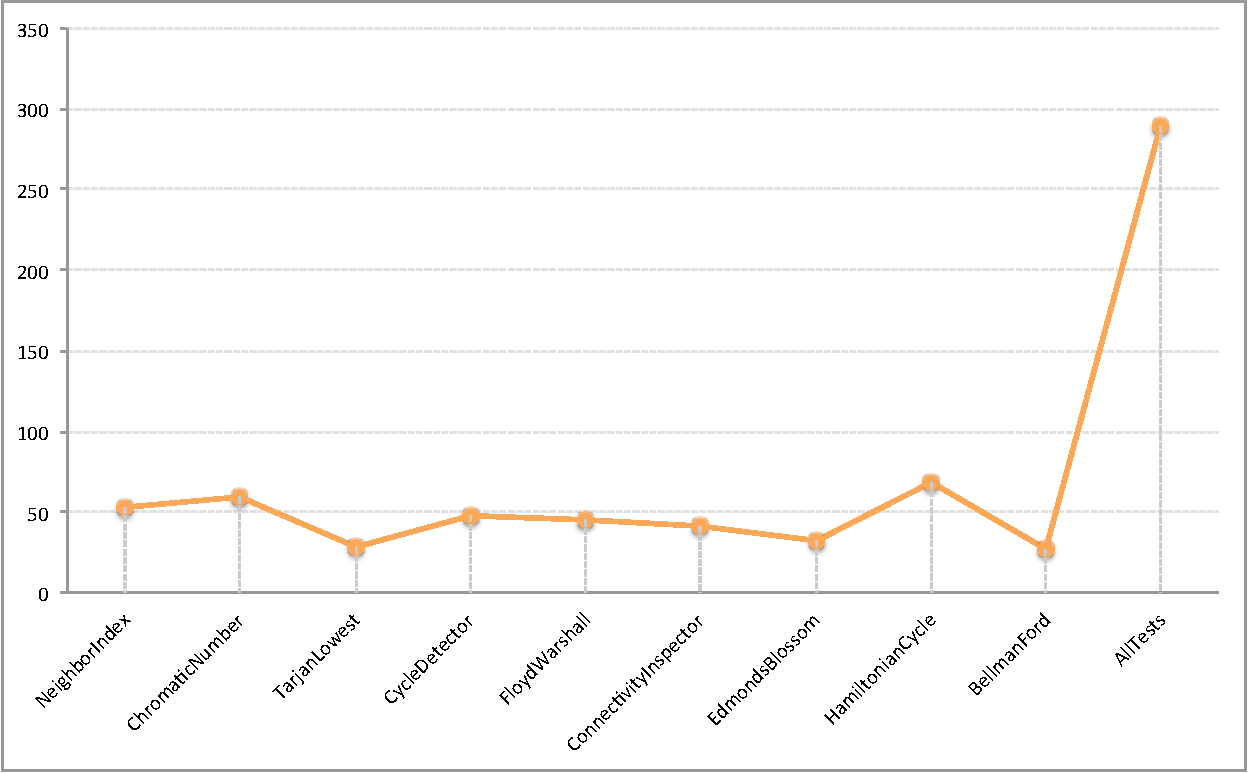
\includegraphics[width=0.8\textwidth]{./Images/tests.pdf}
  \caption{Coverage results of 10 random test cases.}
\label{results}
%\end{minipage}%
%\hspace{0.1cm}
%\begin{minipage}[b]{1\linewidth}
%\centering
% 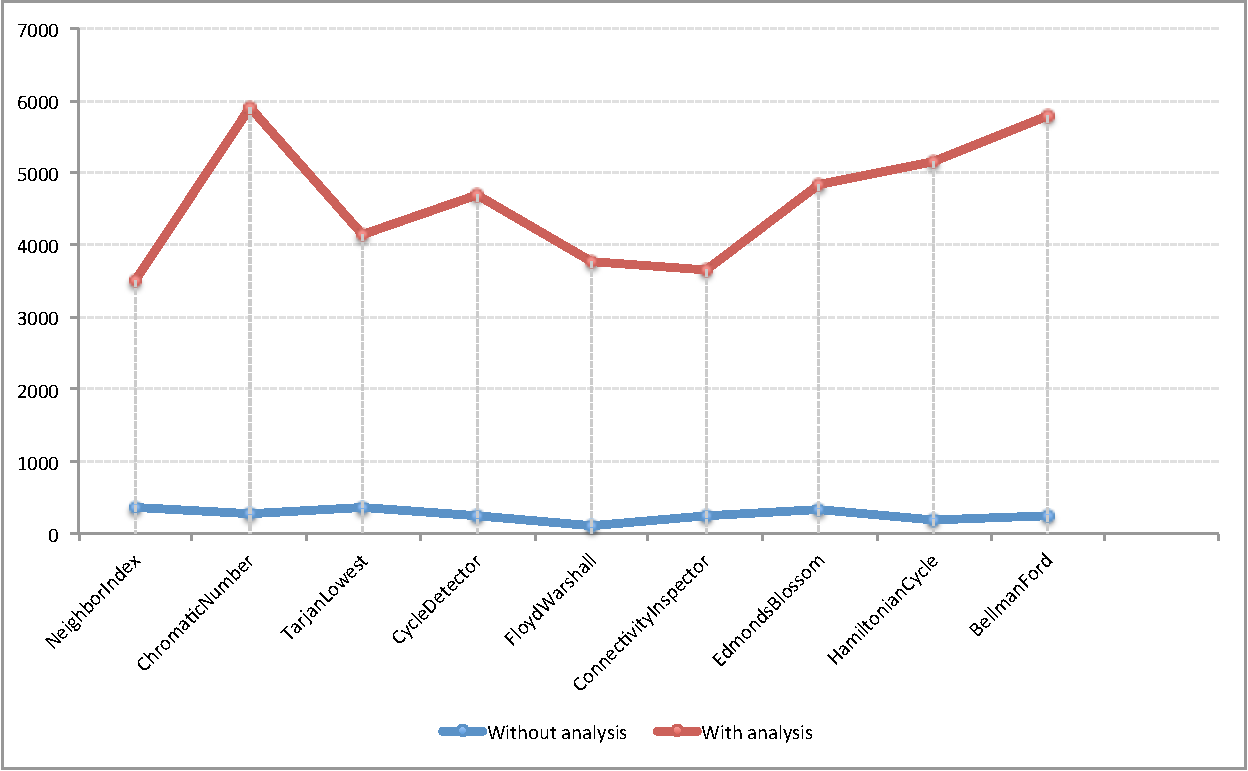
\includegraphics[width=0.95\textwidth]{./Images/overhead.pdf}
% \caption{Time overhead.}
%\label{time}
%\end{minipage}%
%}%

\end{figure}



%\begin{minipage}{0.5\textwidth}
%\begin{figure}[H]
%  \begin{center}
%   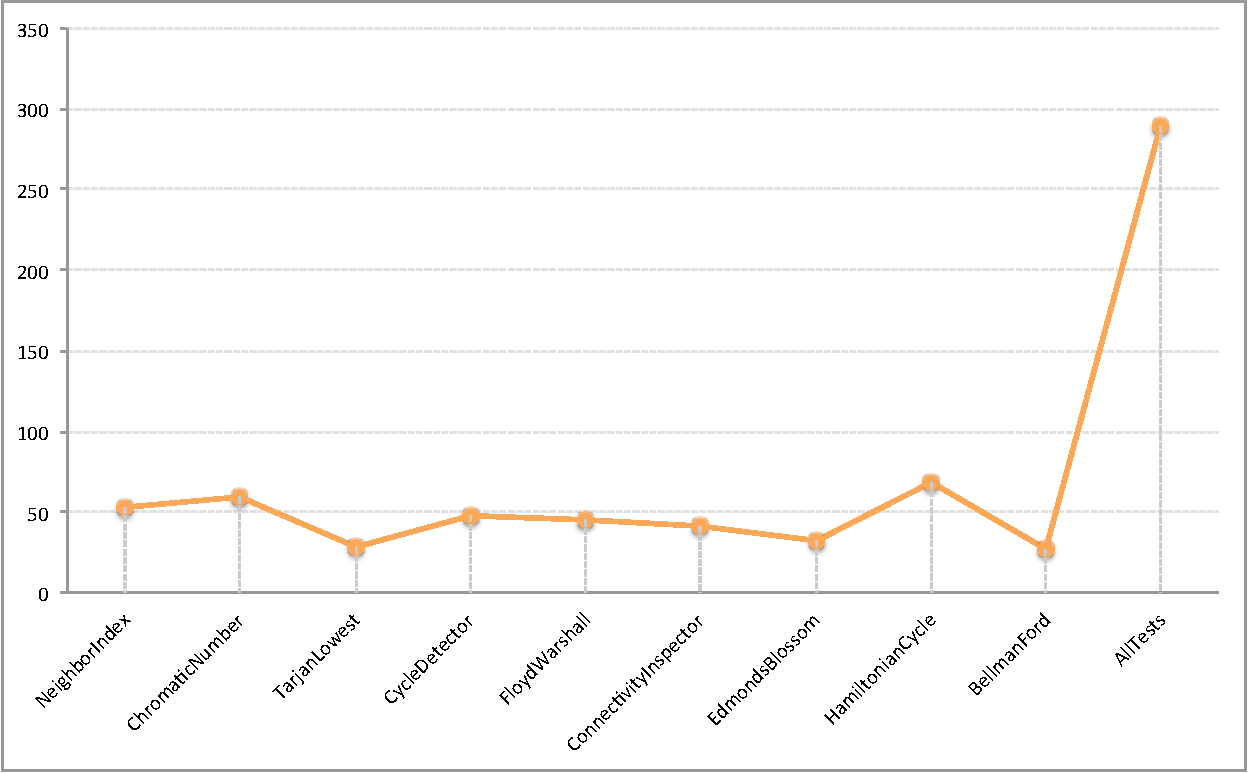
\includegraphics[width=\textwidth]{./Images/tests.pdf}
%   \caption{Coverage results of 10 random test cases.}
%  \label{results}
%  \end{center}
% \end{figure}
% \end{minipage}
% \begin{minipage}{0.5\textwidth}
%\begin{figure}[H]
%  \begin{center}
%   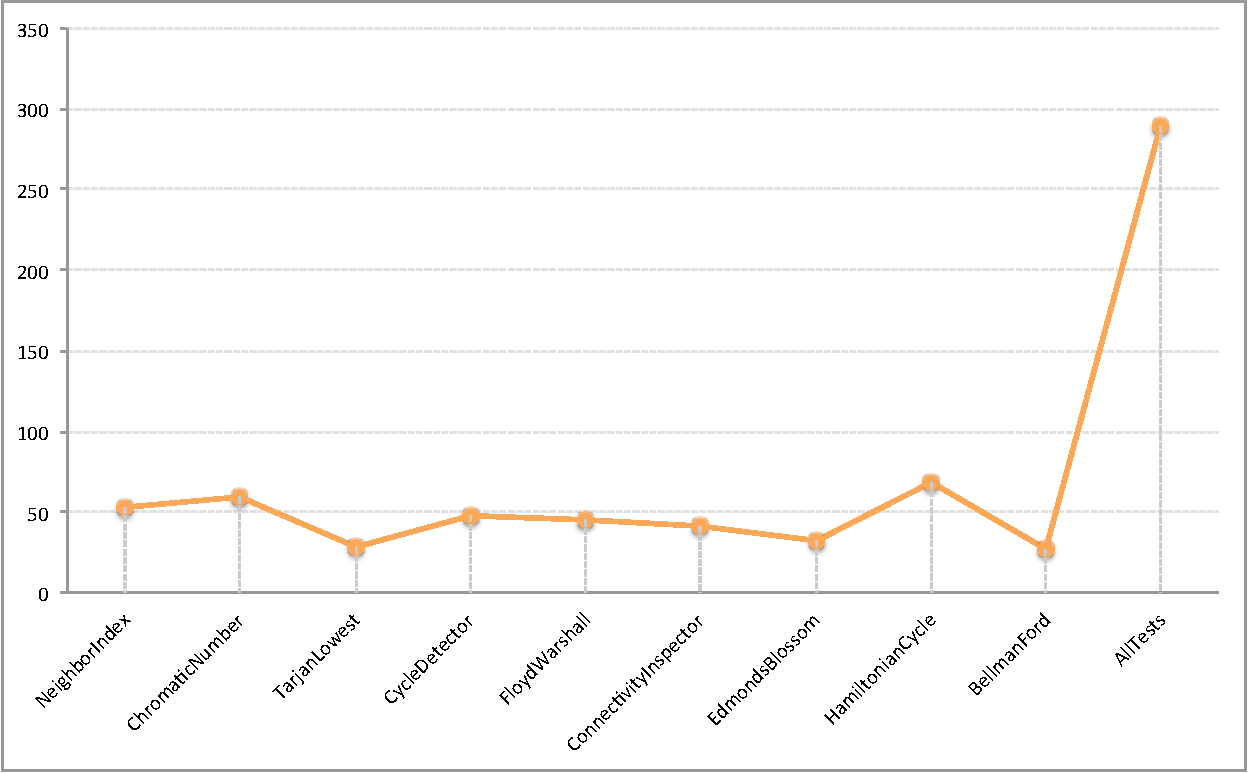
\includegraphics[width=\textwidth]{./Images/tests.pdf}
%   \caption{Coverage results of 10 random test cases.}
%  \label{results}
%  \end{center}
% \end{figure}
% \end{minipage}

%% menzionare che certe coppie non vengono calcolate?
\begin{figure}[htb]
  
\centering
%\centering
%\makebox[0pt][c]{%
%\begin{minipage}[b]{1\linewidth}
%\centering
%  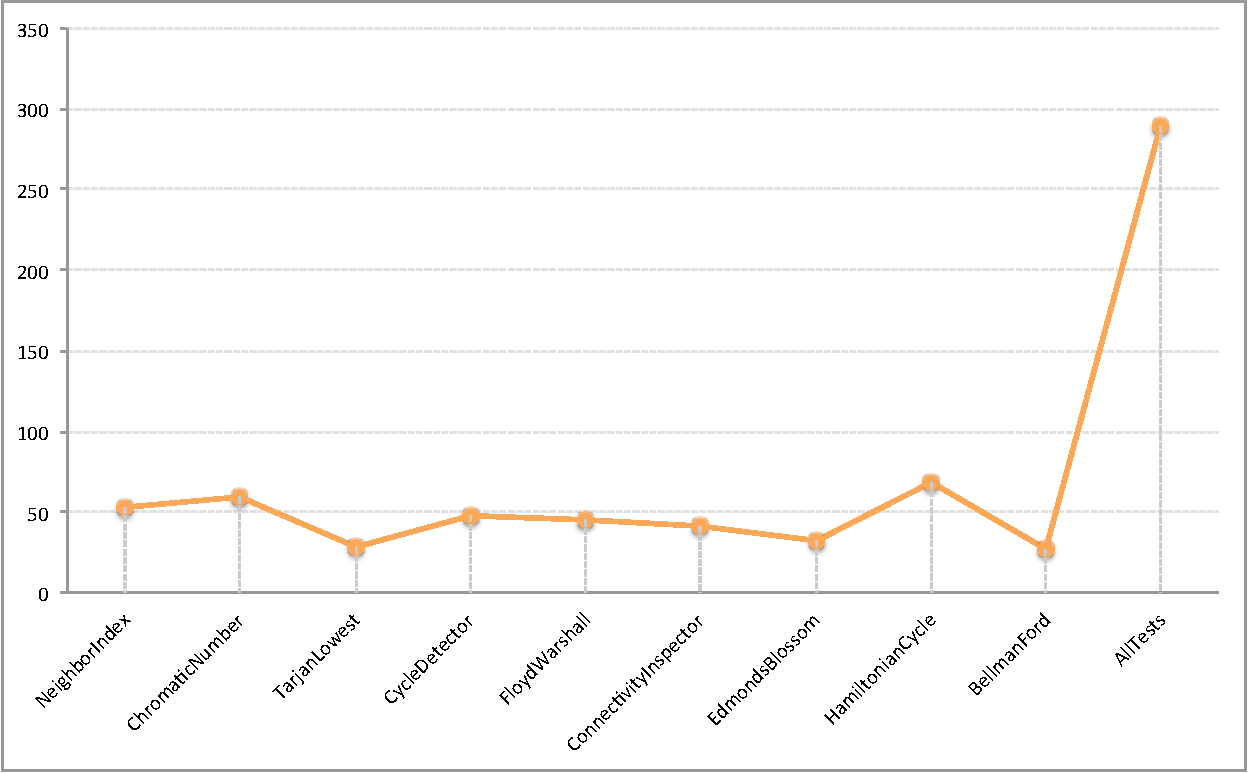
\includegraphics[width=0.6\textwidth]{./Images/tests.pdf}
%  \caption{Coverage results of 10 random test cases.}
%\label{results}
%\end{minipage}%
%\hspace{0.1cm}
%\begin{minipage}[b]{1\linewidth}
\centering
 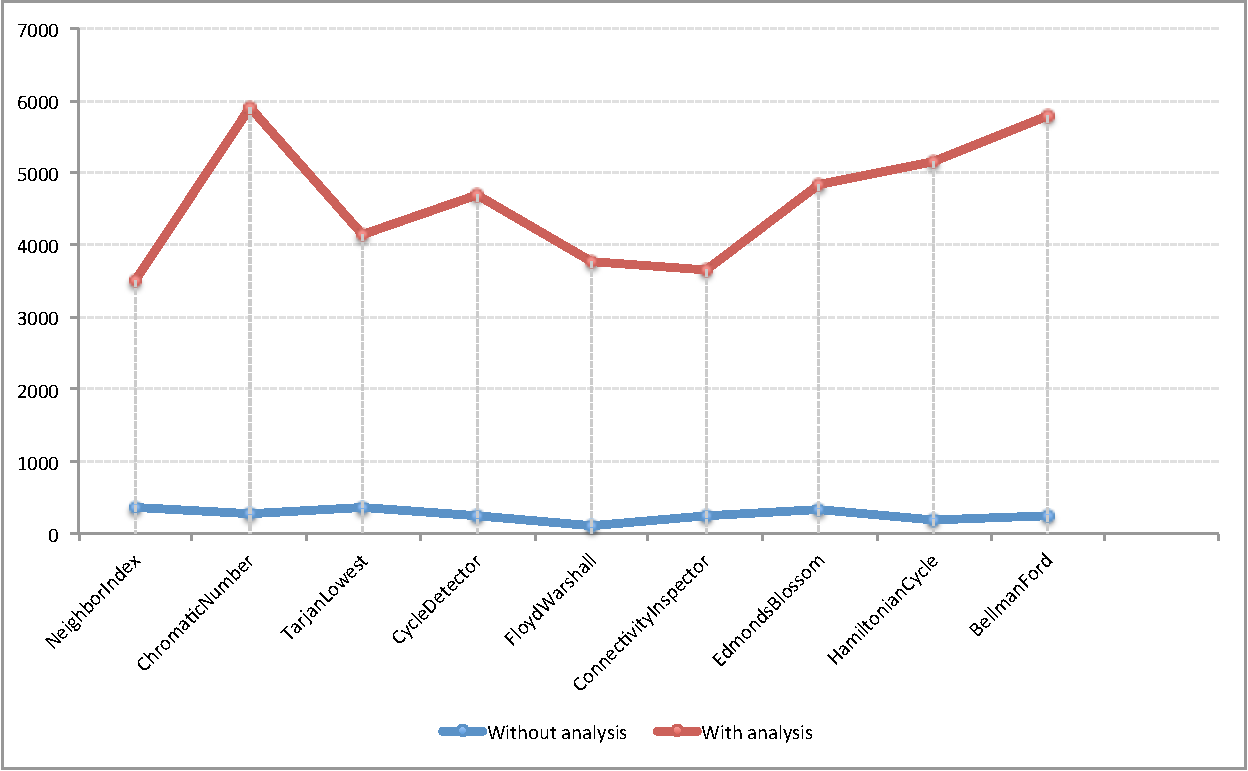
\includegraphics[width=0.8\textwidth]{./Images/overhead.pdf}
 \caption{Time overhead.}
%\label{time}
%\end{minipage}%
%}%

\end{figure}


